\section{}
\subsection{}
Nodes:
\[\{(x_1, x_2, x_3, x_4): x_1,x_2,x_3,x_4 \in \{1,2,3,4\} \setbr \forall i \forall j (x_i\neq x_j)\}\]
Links: 
\[
    (x_1 \ldots x_{i-1}, \alpha, \beta, x_{i+2} \ldots)\sim (x_1 \ldots x_{i-1}, \beta, \alpha, x_{i+2} \ldots)
\]

\subsection{}
We can observe that in bubble sort we require the most swaps to reverse a list e.g.
\[1234 \rightarrow 4321\]
This requires a minimum of 6 swaps.

We will now prove that a reversed list requires the most swaps in bubble sort.
We will prove this for the sequence $1234$, however it generalizes trivially.
By looking at each of the 6 possible ordered pairings of numbers in the sequence we can see that each of the pair is not in the desired order. 
\[ (1,2) (1,3) (1,4)\\
    (2,3) (3,4)\\
    (3,4)
\]

We can observe that each swap operation will flip the order of one pair whilst leaving the others untouched. 
Therefore, we have a lower bound of 6 swaps in the case of a revered list. 

A swapping scheme can also be provided for the revered list case: 
\[
    1234, 2134, 2314, 2341, 3241, 3421, 4321
\]
Giving us a upper bound and therefore proving 6 is swaps is the maximal case.

As $B_4$ models the swapping scheme in bubble sort we can see that the diameter will be the maximal number of swaps required, of which we know is 6 for the revered list.

Therefore, the diameter of $B_4$ is 6.

\subsection{}
We can calculate the number of nodes $B_4$ would have if it was a Moore graph.
We know that $\delta_0 = 3$ and $h=6$

\begin{align*}
&1+\delta_0 + \delta_0(\delta_0-1)+\ldots+\delta_0(\delta_0-1)^{h-1} \\
    =&1 + 3 + 3(3-1)^2 + 3(3-1)^3 + 3(3-1)^4 + 3(3-1)^5\\
    = &1+ 3 + 12 +24+48+96 \\
    = &184
\end{align*}

As $B_4$ only contains 24 nodes it is not a Moore graph.

\subsection{}
Node-disjoint paths from $4312$ to $2314$
\begin{align*}
    &4312 \rightarrow 3412 \rightarrow 3142 \rightarrow 3124 \rightarrow 3214 \rightarrow 2314 \\
    &4312 \rightarrow 4321 \rightarrow 4231 \rightarrow 2431 \rightarrow 2341 \rightarrow 2314\\
    &4312 \rightarrow 4132 \rightarrow 1432 \rightarrow 1342 \rightarrow 1324 \rightarrow 1234 \rightarrow 2134 \rightarrow 2314
\end{align*}

We can see that for any pair of nodes in the graph there cannot be more than 3 node-disjoint paths in $B_4$ as both the source and sink only have degree 3. 

As $B_4$ is symmetric both rotationally and along the vertical axis we can say there are 3 node disjoint paths for both $3214 \rightarrow 4312$ and $1234 \rightarrow 4231$.
The 3 node-disjoint paths for $3214 \rightarrow 4312$ can be obtained by reflecting the $4312\rightarrow 2314$ paths in the vertical axis.
Likewise the 3 node-disjoint paths for $1234 \rightarrow 4231$ can be obtained by roating the 3 node-disjoint paths of $4312\rightarrow 2314$ $120$ degrees clockwise. 

\subsection{}

\newcommand{\ls}{\texttt{label-swap}\xspace}
We will first define and prove the validity of the \ls automorphism.
Then we will constrict this automorphism to create the \texttt{neighbour label-swap} automorphism.
And finally, we will prove a series of the \texttt{neighbour label-swap} automorphisms can map any node to any other node thus proving that $B_4$ is node-symmetric.

We will start by generalising the labeling of our nodes.
Given we will often be focusing on a single node $X$, we will say $X=(x_0, x_1, x_2, x_3)$ where $x_0,x_1,x_2,x_3\in\{1,2,3,4\}$ and $x_0, x_1, x_2, x_3$ are distinct.
We can then label the remaining nodes of $B_4$ according to the values of $x_0, x_1, x_2, x_3$.

The \ls automorphism takes parameters $i, j$ such that $0 \leq i <j \leq 3$, then swaps the position of $x_i$ and $x_j$.
 For example $(x_0, x_1, x_2, x_3)$ and $(x_1, x_0, x_3, x_2)$ under \ls with $i=0$ and $j=3$ would be $(x_3, x_1, x_0, x_3)$ and $(x_1, x_3, x_0, x_2)$ respectively.
 Formalising this, \ls is a function $\Phi: V, i, j \rightarrow V$ where $V$ is the set of nodes and $i,j$ our the indices we will swap.
 We will also define the helper function $f: L, i, j \rightarrow L$ where $L={0,1,2,3}$.
 \[ \Phi((y_0, y_1, y_2, y_3), i,j )=(f(y_0,i,j), f(y_1,i,j), f(y_2,i,j), f(y_3,i,j))
\]
\[ f(y_\alpha, i, j) = 
    \begin{cases} 
      y_j & \alpha=i \\
      y_i & \alpha=j \\
      y_\alpha & \text{Otherwise} 
   \end{cases}
\]
By definition \ls is a permutation of the graph.

We next look to prove that \ls is channel preserving.
For any general vertex $X=(x_0, x_1, x_2, x_3)$ we know that it is connected via 3 channels to 3 other vertices. 
Namely it is connected to 3 neighbours:
\begin{align*}
N_1 &= (x_1, x_0, x_2, x_3)\\
N_2 &= (x_0, x_2, x_1, x_3)\\
N_3 &= (x_0, x_1, x_3, x_2)
\end{align*}
Applying label swap to $X$ we calculate $Y=\Phi(X)$.
We can say that $Y=(y_0, y_1, y_2, y_3)$.
Using the definition of $\Phi$ we can see that $y_\alpha = f(x_\alpha)$ and that all $y_\alpha$ are distinct because $f$ is bijective.
Applying label swap to each of the neighbours
\begin{align*}
\Phi(N_1) &= (f(x_1), f(x_0), f(x_2), f(x_3))=(y_1, y_0, y_2, y_3)\\
\Phi(N_2) &= (f(x_0), f(x_2), f(x_1), f(x_3))=(y_0, y_2, y_1, y_2)\\
\Phi(N_3) &= (f(x_0), f(x_1), f(x_3), f(x_2))=(y_0, y_1, y_3, y_2)
\end{align*}
We can observe that the relationship between $Y, \Phi(N_1), \Phi(N_2), \Phi(N_3)$ is equivalent to that of $X, N_1, N_2, N_3$, therefore \ls preserves neighbours and hence also preserves channels.
As \ls is a permutation of $B_4$ and channel preserving it is an automorphism.

We can restrict \ls to \texttt{neighbour label-swap} (\texttt{nls}) by imposing the restriction that $j\leftarrow i+1$ i.e. we can only swap the labels of neighbouring values.
As we have proven that \ls is an automorphism and we can see that \texttt{nls} contains a subset of possible mappings in \ls, we know that \texttt{nls} must also be an automorphism.

Now we will prove that any node can be mapped onto any other node using a series of \texttt{nls}.
We can construct a graph to analyse if we can transition from any $(x_0, x_1, x_2, x_3)$ to a permutation of $x_0, x_1, x_2, x_3$ using only neighbour swaps.
We will use the index of each $x_i$ to label every node, so $(x_i, x_j, x_k, x_l)$ will be represented as the node $(i,j,k,l)$.
Using \texttt{nls} there is an edge between each node if a single neighbouring pair have swapped.
This is in-fact the exact definition of $B_4$.

Hence, by virture of $B_4$ being fully connected we can apply a series of \texttt{nls} to map any node onto any other node. Therefore $B_4$ is node symmetric.

% 5
\section{}
\subsection{}
We can perform a single node scatter in $\mathcal{K}$ using $H$  by simply routing the traffic around $H$.
For effciency sake will will route traffic round $H$ in both directions similtaiously.
Let us symbolically define $H$ as follows:
\[
H = h_{\text{start}}, h_1, h_2, \ldots, h_{62}, h_{63}, h_{\text{start}}
\]
On the first clock tick we will send a message for $h_{31}$ to $h_1$ and $h_{32}$ to $h_63$.
In the next clock tick $h_1$ forwards all messages onto $h_2$ likewise for $h_{63}$ and $h_{62}$.
We also send the message for $h_{30}$ to $h_1$ and similarly for $h_{33}$ and $h_{63}$.
And so on until every message has been sent.

Every node will only require a buffer size of 1 as it only every recieves messages from one source and will forward them straight away.
This routing transmits $2$ new messages every clock tick and needs to transmit a total of $63$ messages, hence this single node scatter will take $\lceil 63/2 \rceil=32$ clock cycles.


\subsection{}
Let us first derive the embedding of $Q^4_3$ into $Q_3$.
Our embedding will firstly group the nodes of $Q_3^4$ into sets and then map these sets onto nodes of $Q_3$.

We know that $Q^4_3$ has 64 nodes and $Q_3$ has 8 nodes, so we will construct 8 sets of size 8.
To do this we will use $H$.
We will take the 1st 8 nodes in $H$ and group them, then the 2nd 8 and so on.
By construction of $H$ we can label each of these 8 sets with the index of the 1st node added to each set.
These are the sets $S_{(0,0,0)}, S_{(0,2,0)}, S_{(0,2,1)} S_{(0,0,1)} S_{(0,0,2)} S_{(0,2,2)} S_{(0,2,3)} S_{(0,0,3)}$.
Note that the first dimension in each label is $0$ for all sets, hence for convenience it will be omitted from now on. 

We can now draw $H$ as follows.
\begin{center}
    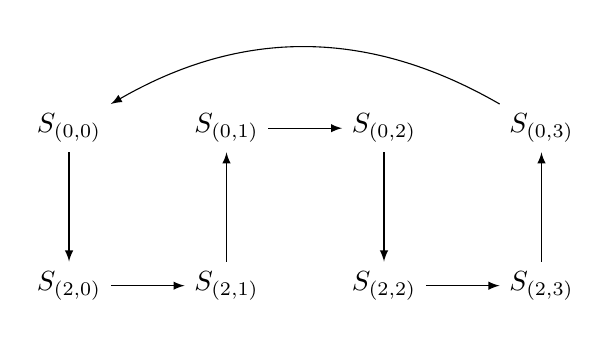
\begin{tikzpicture}[auto, xscale = 2, yscale = 2]
        \node (s0) at (0,1) {$S_{(0,0)}$};
        \node (s1) at (0,0) {$S_{(2,0)}$};
        \node (s2) at (1,0) {$S_{(2,1)}$};
        \node (s3) at (1,1) {$S_{(0,1)}$};
        \node (s4) at (2,1) {$S_{(0,2)}$};
        \node (s5) at (2,0) {$S_{(2,2)}$};
        \node (s6) at (3,0) {$S_{(2,3)}$};
        \node (s7) at (3,1) {$S_{(0,3)}$};
        
        
        \draw[-latex] (s0) to node[pos=0.3] {} (s1);
        \draw[-latex] (s1) to node[pos=0.3] {} (s2);
        \draw[-latex] (s2) to node[pos=0.3] {} (s3);
        \draw[-latex] (s3) to node[pos=0.3] {} (s4);
        \draw[-latex] (s4) to node[pos=0.3] {} (s5);
        \draw[-latex] (s5) to node[pos=0.3] {} (s6);
        \draw[-latex] (s6) to node[pos=0.3] {} (s7);
        \draw[-latex] (s7) edge[bend right] node [left] {} (s0);
    \end{tikzpicture}
\end{center}

A mapping onto $Q_3$ while ensuring every channel in $H$ is either within a node or a single channel is now simple.
We will refer to the nodes $(1, x, y)$ in $Q_3$ as the top $Q_2$ and $(0, x, y)$ as the bottom $Q_2$.
We will map $S_{(0, x)}$ to the top $Q_2$ and $S_{(2, x)}$ to the bottom $Q_2$.
Within each $Q_2$ we will map: 
$S_{(x, 0)}$ to $(0,0)$; 
$S_{(x, 1)}$ to $(0,1)$; 
$S_{(x, 2)}$ to $(1,1)$; 
and $S_{(x, 3)}$ to $(1,0)$.
That completes our embedding.

With this embedding it is easy to implement a single node scatter within our $Q_3$ using the same routing as we did in Q5a.
However now we experience the patten that we transit though 8 internal channels within a set before using 1 physical channel to move set (aka node in $Q_3$).

As every path taken in the single node scatter in Q5a has been mapped onto a path with length either 0 or 1 there should be no prominent additional overheads to a single node scatter in our $Q_3$.
Excluding the obvious overhead of every node in $Q_3$ having a load of 8.

% 6
\section{}
\subsection{}
For $Q_4$ we have the vertex set
\[
    V_4 = \{(x_0,x_1,x_2, x_4): x_0, x_1, x_2, x_3 \in \{0,1\}\}    
\]
And $Q_3$ we have the vertex set
\[
    V_3 = \{(y_0,y_1,y_2): y_0, y_1, y_2 \in \{0,1\}\}    
\]
Our embedding $\Phi: V_4 \rightarrow V_3$ will be:
\[\Phi((x_0, x_1, x_2, x_3))=(x_1, x_2, x_3)\]

Therefore every vertex is $Q_3$ will have a load of 2 as 2 vertices from $Q_4$ have been mapped to it.
Likewise every channel will have congestion 2 as there are 2 channels mapped to it.
Both the load and congestion greater than 1 are overheads introduced by this embedding.
One mechanism that needs to be introduced to facilitate this embedding is an internal channel within a node to connect $(0, x_1, x_2, x_3)$ and $(1, x_1, x_2, x_3)$.
As each node is a processor we can implement such a channel in software.
This will however introduce an additional overhead on our processors.

\subsection{}
We will keep track of how many new nodes we have already been added $n$.
The binary encoding of $n$ is $(n_0, n_1, n_2)$ where $n_0$ is the most significant bit.
We will call our growing network $C'$, where initially $C'\leftarrow C$, we will also name the set of new nodes as $C^+$.
A few identities we have are $|C^+|=n$ and $C \cup C^+ = C'$.

To add the first new node $k$ we begin by noting that $n=0$, then:
\begin{enumerate}
\item $k$ will take the node id $(1, n_0, n_1, n_2)$.
\item Calculate all the neighbours $k$ (all labels that differ by one bit).
\item Connect $k$ to the nodes currently running the neighbour processes. 
Some neighbours might be running on their own node in $C^+$.
Others may not and still be embedded in $C$.
It is a simple calculation with comparison to $n$ to determine where the neighbour is.
Note that $k$ is connected but has not been switched on yet.
\item Unassociate node $(n_0, n_1, n_2)$ in $C$ with $(1, n_0, n_1, n_2)$ leaving that node only running $(0, n_0, n_1, n_2)$.
To the network  $(1, n_0, n_1, n_2)$ appears to be faulty.
\item Update all routing information on every other node in $C'$ to make them aware of $k$.
\item Turn $k$ on.
\end{enumerate}
Once the first node has been added we can just repeat these steps to add the remaining node.
However, we will also add an additional tidying step to remove obsolete channels.
\begin{enumerate}[resume]
  \item Remove all the now-unused channels between $x\sim(n_0, n_1, n_2)$ where $x\in C$. i.e. all channels between new nodes and $(n_0, n_1, n_2)$ should be removed unless that new node is $k$.
\end{enumerate}


